\chapter{Program Installation}

The operating system used for the project is Raspbian Jessie. To simplify installation, the SD card of the Raspberry Pi was flashed with an OS installer containing Raspbian Jessie, called NOOBS (New Out Of the Box Software) \cite{rpi3noobs}. When starting up, the loading screen will look typically like Figure \ref{rpi3noobs}. The version of NOOBS used was version 1.9.2, with a release date of 27/5/2016. 

\begin{figure}[H]
	\centering
	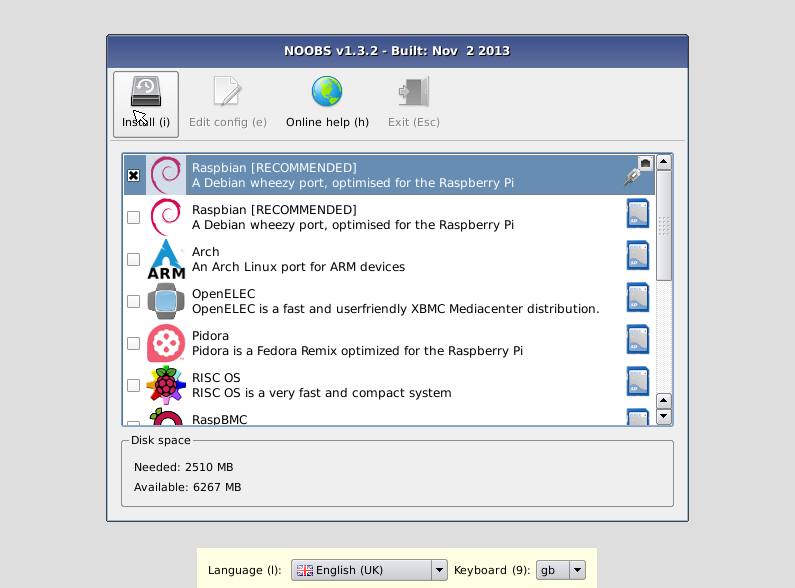
\includegraphics[width=\linewidth]{noobs.png}
	\caption{NOOBS (New Out Of the Box Software) Initial Installation Screen \cite{rpi3noobs}}
	\label{rpi3noobs}
\end{figure}

Aside from using NOOBS for the OS installation, it is possible to download the Raspbian Jessie image from the official Raspberry Pi website, unzip the image file, and copy it to the SD card. However, NOOBS was used specifically for its convenience, since it is necessary to obtain disk imager utilities on Windows for this method. Nevertheless, the choice of installation approach does not in any way affect the functionality of the OS after it has been loaded.  

\section{Operating System - Raspbian Jessie}
\label{appraspbianjessie}






\begin{lstlisting}
sudo apt-get update
sudo apt-get install tightvncserver
sudo apt-get install xtightvncviewer
sudo apt-get install arduino
sudo apt-get install python-matplotlib
\end{lstlisting}





\section{Code}

\subsection{Arduino Code for Thermistor}
\label{arduinothermistor}

\begin{lstlisting}[language=c]
/*
AnalogReadSerial
Reads an analog input on pin 0, prints the result to the serial monitor.
Attach the center pin of a potentiometer to pin A0, and the outside pins to +5V and ground.

This example code is in the public domain.
*/

#include <math.h>
#include <stdlib.h>
#include <stdio.h>

double T; 
double TK; 
double lnratio; 
double a, b, c, d; 

// the setup routine runs once when you press reset:
void setup() {
	// initialize serial communication at 9600 bits per second:
	Serial.begin(9600);
}

// the loop routine runs over and over again forever:
void loop() {
	// read the input on analog pin 0:
	double sensorValue = analogRead(A0);
	// print out the value you read:
	a = 3.3540154e-3;
	b = 2.5627725*pow(10,-4);
	c = 2.0829210*pow(10,-6);
	d = 7.3003206*pow(10,-8);
	
	// lnratio = log(sensorValue/(1023-sensorValue));
	for (double i=1;i<1024;i++) {
		lnratio = log(i/(1024-i));
		T = 1/(a+b*(lnratio)+c*pow(lnratio,2)+d*pow(lnratio,3)); 
		TK = T-273.15; 
		
		Serial.println(TK); 
		//Serial.print(' '); 
		//Serial.println(sensorValue);
		
		delay(1);}        // delay in between reads for stability
}
\end{lstlisting}

\subsection{MATLAB ECG Simulation}
\label{ecgsimulationcode}

The simulated ECG signal in Figure \ref{ecgsim} in Section \ref{simulation} was obtained by running the following code in MATLAB.

\begin{lstlisting}
>>ECGwaveGen(70,5,500,2500)
\end{lstlisting}

The ECGwaveGen.m file below was obtained from physionet.org \cite{ecgsimulation}.

\begin{lstlisting}[language=Matlab]
function [QRSwave]=ECGwaveGen(bpm,duration,fs,amp)
%[QRSwave]=ECGwaveGen(bpm,dur,fs,amp) generates an artificial ECG/EKG waveform
%    Heart rate (bpm) sets the qrs event frequency (RR interval). 
%    Duration of the entire waveform (dur) is in units of seconds.
%    Sample frequency (fs) sets the sample frequency in Hertz. 
%    Amplitude (amp) of the QRS event is measured in micro Volts. The
%    waveform consists of a QRS complex and a T-wave. No attempt to 
%    represent a P-wave has been made.
%     
%    There are two additional parameters that can be changed from within the function.
%    They are the parameters that set the QRS width (default 0.1 secs) and the t-wave 
%    amplitude (default 500 uV).

%Created January 22, 2001 by Floyd Harriott, primary email (fharriott@stellate.com), secondary email (fsh@po.cwru.edu)
%Modified March 19, 2002 by Floyd Harriott, extended default duration so that default settings produce a QRS event rather than 
%   an error. Allows for the random insertion of PVCs.  This file must be edited to include PVCs.

%Algorithm is based in part on the jounal article:
%Ruha, Antti and Seppo Nissila, "A Real-Time Microprocessor QRS Detector System with a 1-ms Timing Accuracy
%      for the Measurement of Ambulatory HRV", IEEE Trans. Biomed. Eng. Vol. 44, No. 3, 1997
%The artificial ECG signal they describe is based on the recommendations in the Association for the Advancement
%of Medical Instrumentation (AAMI) "Standard for Cardiac Monitors, Heart Rate Meters and Alarms (draft), Aug. 1981
%Feel free to make modifications, corrections and or suggestions.

if (exist('fs') ~= 1)  fs=  200;   end  %default value, Hz
if (exist('bpm') ~= 1)  bpm =  72;   end %default value, beats per minute
if (exist('amp') ~= 1)  amp = 1000;   end %default value, micro volts
if (exist('duration') ~= 1)  duration =  (60/bpm-0.35)+60/bpm+1/fs; end  %default value gives one cycle, seconds

global t_line; %seconds
global sample_freq; % always equal to fs


%Changeable Parameters
d=0.1; %.07 to .120 seconds, QRS width
at=500; %amplitude of t-wave, 400 to 1200 uv

%Should not touch
org_amp=amp;
sample_freq=fs; %duplicated simply to make a global version
RR=(60/bpm); %RR interval, seconds
d1=0.4375*d;
d2=0.5*d;
d3=d-(d1+d2);
dt=0.180; %width of t wave, seconds
qt=0.35; %time from beginning of QRS to end of t-wave
t_line=0:1/fs:duration; %time line, seconds
QRS_wave=zeros( size(t_line) ); %QRS waveform
deadspace=RR-qt; %time between t-wave and next QRS
if deadspace < 0 
err_msg=['Bpm must be equal to or less than ' int2str(60/qt) ' inorder to fit one cycle.'];
error(err_msg); 
end


%Calculate PVC parameters and segment
PVCchance=0.1; %How often does PVC happen., percent eg. 0.1=10%
PVCamp=amp;    %PVC amplitude, eg. same as normals (amp)
earlyfactor=0.25; %percentage, how much early should PVC happen then normal RR interval
PVCwidth=0.12; %seconds, QRS width of PVC, usually .12 to .17
PVCseg=[QRSpulse(d,60/((1-earlyfactor)*RR-0.4375*PVCwidth),fs,RandAmp(org_amp)) QRSpulse(PVCwidth,bpm*(1-earlyfactor),fs,PVCamp) QRSpulse(d,bpm,fs, RandAmp(org_amp))]; %PVC segment
tPVC=size(PVCseg,2)/fs; %amount of time taken up by PVC segment in seconds

t1=deadspace; %Where does the first QRS start? eg deadspace, or 0

%need enough time to display at least one interval.
if (t1+60/bpm+1/sample_freq > duration)
err_msg=['The waveform length (duration) must be more than ' sprintf('%.2f%',t1+60/bpm+1/sample_freq) ' second(s) in order to display one QRS event.'];
error(err_msg);
end


%GENERATION LOOP
while ( t1+60/bpm+1/sample_freq <= duration) %space to insert another qrs pulse in time line

%amp=RandAmp(org_amp); %random size on qrs event
amp=org_amp;



%Segment 1  (Q-R)
qrs_start=t1;   
t2=t1+d1;
i_t1=time2index(t1); i_t2=time2index(t2);
left=0; right=0.875*amp;
m1=(right-left)/(t2-t1);
QRS1=m1*index2time(i_t1:i_t2)-(m1*t1-left);
QRSwave(i_t1:i_t2)=QRS1;

%Segment 2  (R-?)
t1=t2; t2=t1+d2;
i_t1=time2index(t1); i_t2=time2index(t2);
left=right; right=-.125*amp;
m2=(right-left)/(t2-t1);
QRS1=m2*index2time(i_t1:i_t2)-(m2*t1-left);
QRSwave(i_t1:i_t2)=QRS1;


%Segment 3 bottom_top (?-S) 
t1=t2; t2=t1+d3; 
i_t1=time2index(t1); i_t2=time2index(t2);
left=right; right=0;
if (i_t2-i_t1 >0) %at low sampling freq. there may be no sample for this segment
m3=(right-left)/(t2-t1);
QRS1=m3*index2time(i_t1:i_t2)-(m3*t1-left);
QRS1=QRS1( find(QRS1<=0));
QRSwave(i_t1:i_t1+size(QRS1,2)-1)=QRS1;
elseif i_t2-i_t1==0
m3=(right-left)/(t2-t1);
QRS1=m3*index2time(i_t1:i_t2)-(m3*t1-left);
QRSwave(i_t1)=QRS1(1);
end

%Segment 4, S-T interval
t1=t2; t2=t1+qt+qrs_start-(dt+t2);
i_t1=time2index(t1); i_t2=time2index(t2);
left=right; right=0;

%Segment 5, t-wave
t1=t2; t2=t1+dt;
i_t1=time2index(t1); i_t2=time2index(t2);
t=-1:2/(i_t2-i_t1):1;
QRS1=at*sqrt(1-t.^2);
QRSwave(i_t1:i_t2)=QRS1;

%Segment 6, remaining deadspace
t1=t2; t2=t1+deadspace;
i_t1=time2index(t1); i_t2=time2index(t2);


%Do we insert a PVC here? Roll the die and find out.
insertPVC=rand(1); %uncomment following 5 lines if PVCs are desired.
%if insertPVC<=PVCchance & t2+tPVC+2/sample_freq <= duration %enough space to insert PVC
%   t1=t2; t2=t1+tPVC;
%  i_t1=time2index(t1); i_t2=time2index(t2);
% QRSwave(i_t1:i_t1+size(PVCseg,2)-1)=PVCseg;
%end

%stem(QRSwave); % view ECG waveform
t1=t2; %end of this segment becomes beginning of next segment

end %while loop, appending qrs pulses

%_____________________________________%
function index=time2index(t)
%TIME2INDEX converts time (s) to an index value

global t_line;

indexArray=find(t_line>=t);
index=indexArray(1); 

%_____________________________________%
function time=index2time(i)
%INDEX2TIME converts a time line index to a time value (seconds)
global sample_freq

time=(i-1).*1/sample_freq;


%_____________________________________%
function RAmp=RandAmp(orgAmp)

RAmp=orgAmp+0.4*orgAmp*rand(1);
\end{lstlisting}
